\chapter{Testing}

As with any software engineering project testing is integral to creating a well rounded and robust product that the users actually want to use. Good quality testing helps with keeping the application reliable and should ensure that the end users do not get bombared by a vast array of issues that will ultimately hurt the applications reputation within the market place.

\section{User Testing}

\subsection{Testing community}

\subsection{Test Devices}


\section{Unit Testing}

\section{UI Testing}

\begin{figure}[h]
    \centering
    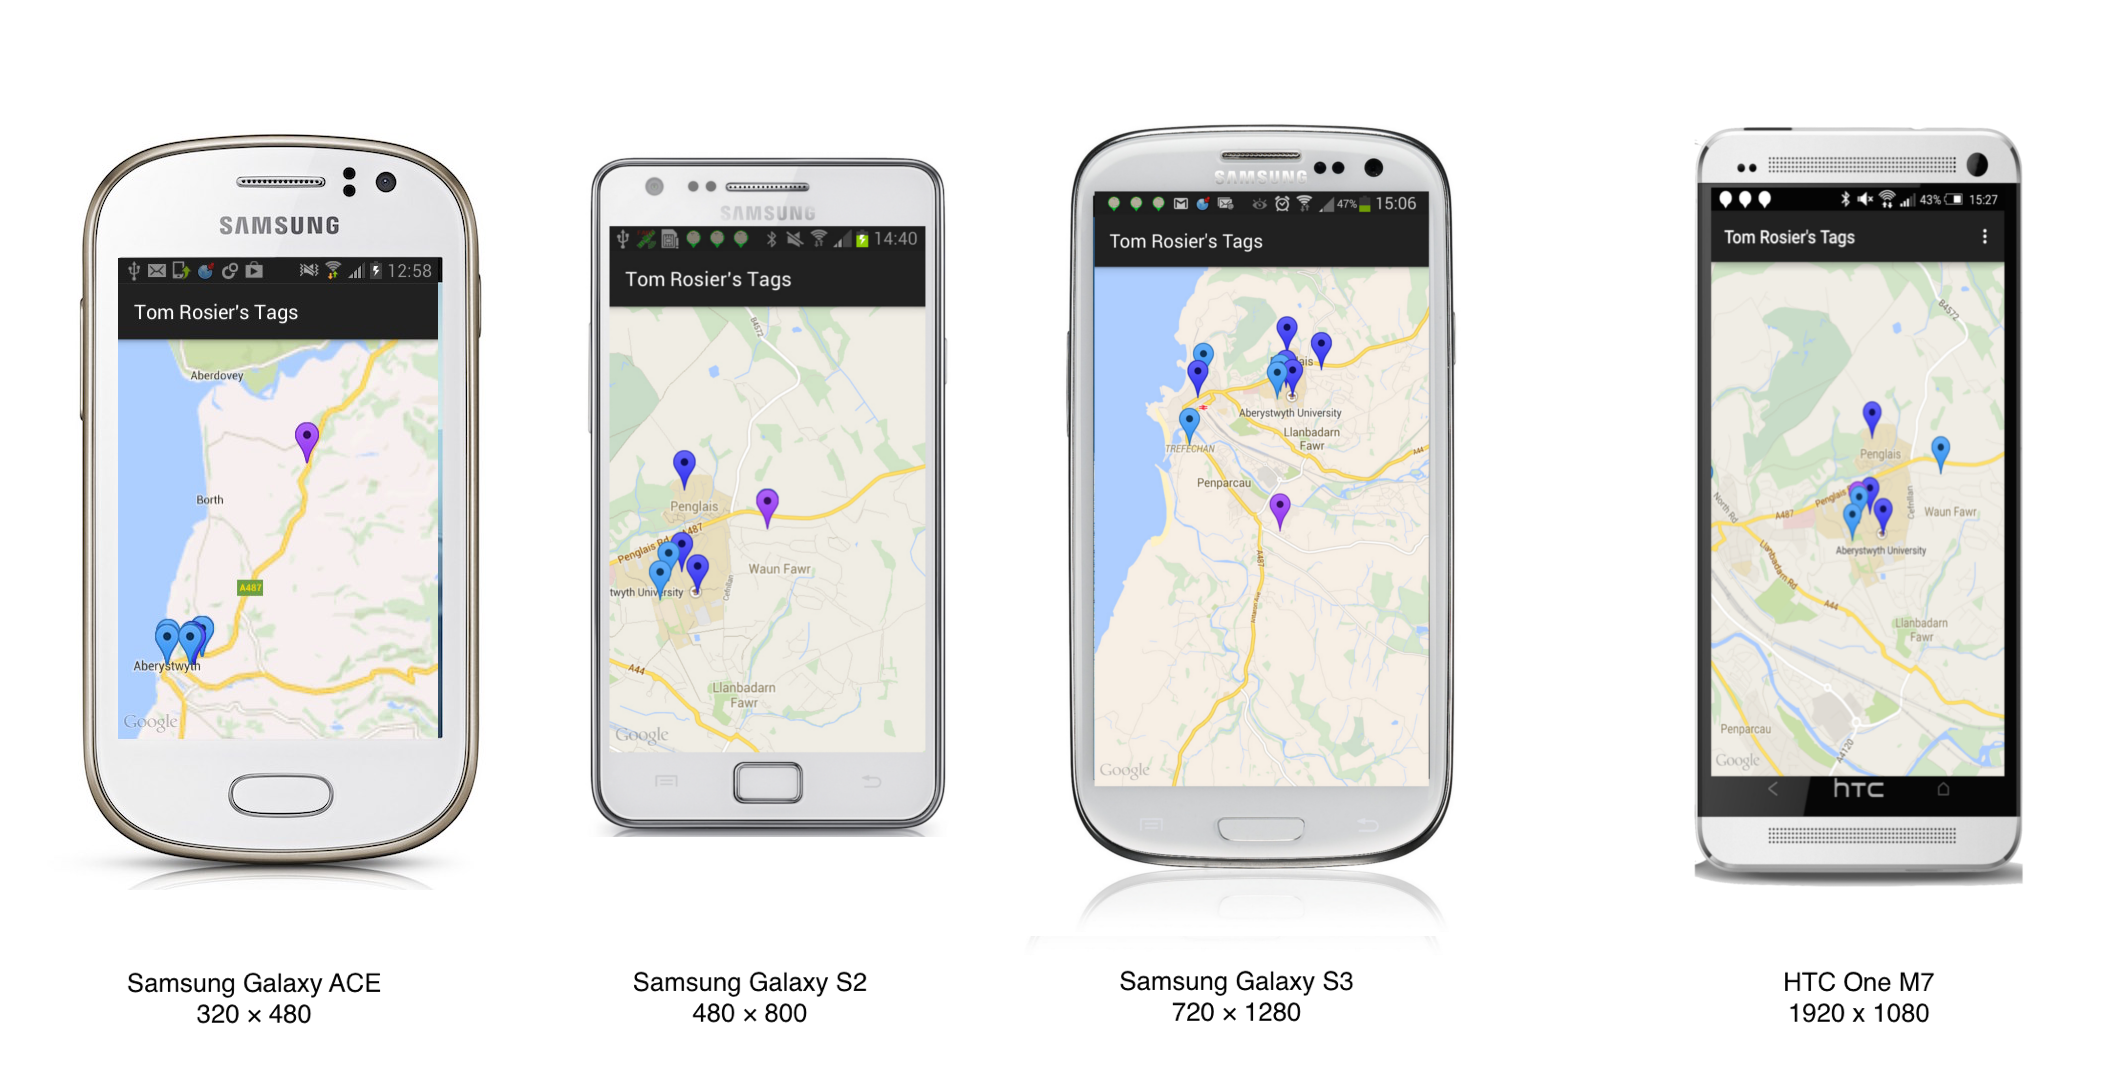
\includegraphics[width=\textwidth]{uiscaling/home}
    \caption{Home activity on different devices}
    \label{fig:ui_scaling_home_image}
\end{figure} 
\noindent

\begin{figure}[h]
    \centering
    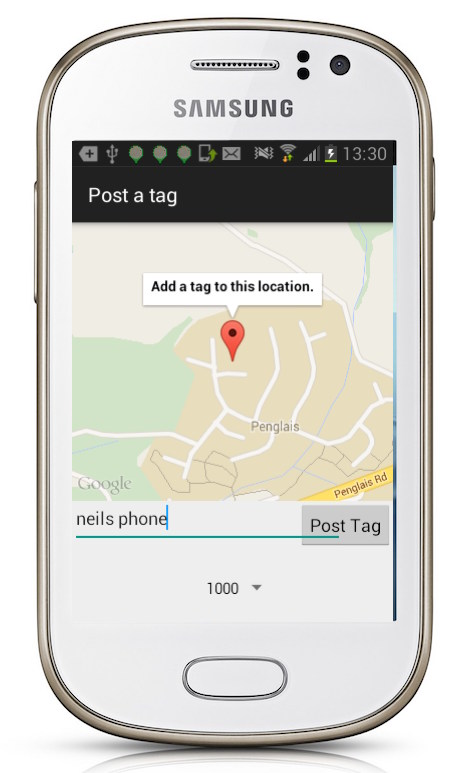
\includegraphics[width=\textwidth]{uiscaling/post}
    \caption{Post message activity on different devices}
    \label{fig:ui_scaling_post_image}
\end{figure} 
\noindent

\begin{figure}[h]
    \centering
    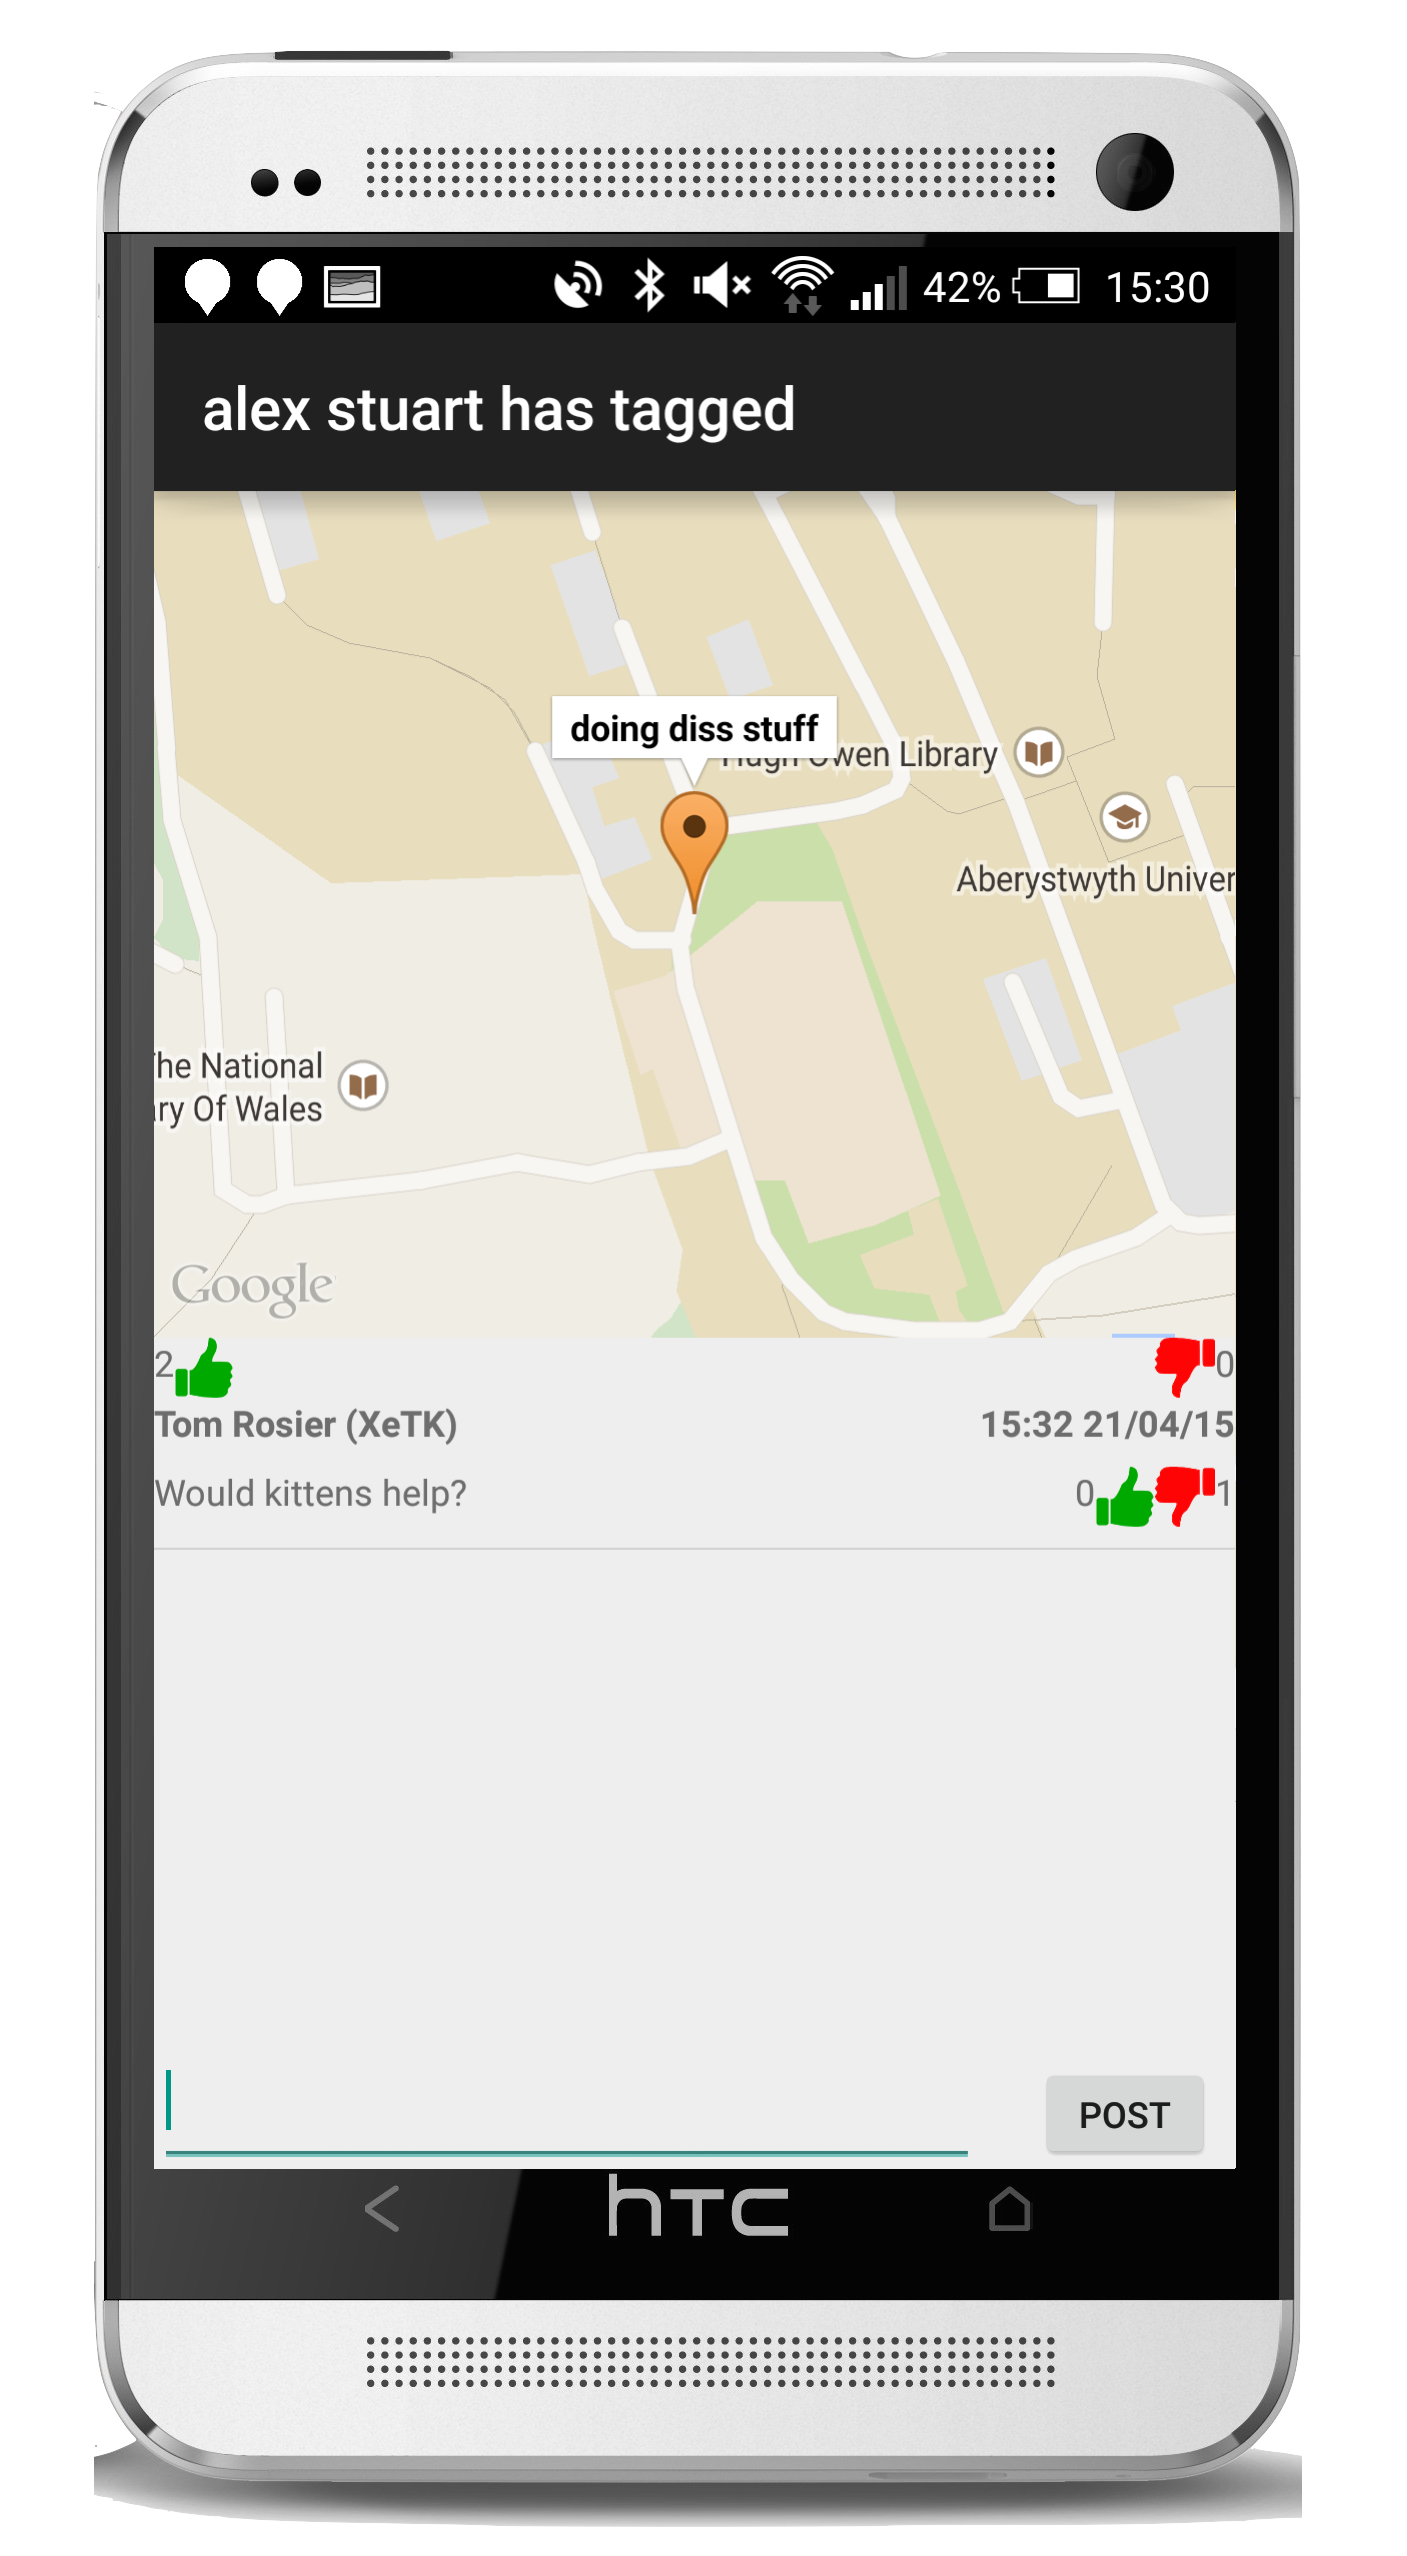
\includegraphics[width=\textwidth]{uiscaling/view}
    \caption{Viewing message on activity on different devices}
    \label{fig:ui_scaling_view_image}
\end{figure} 
\noindent

\begin{figure}[h]
    \centering
    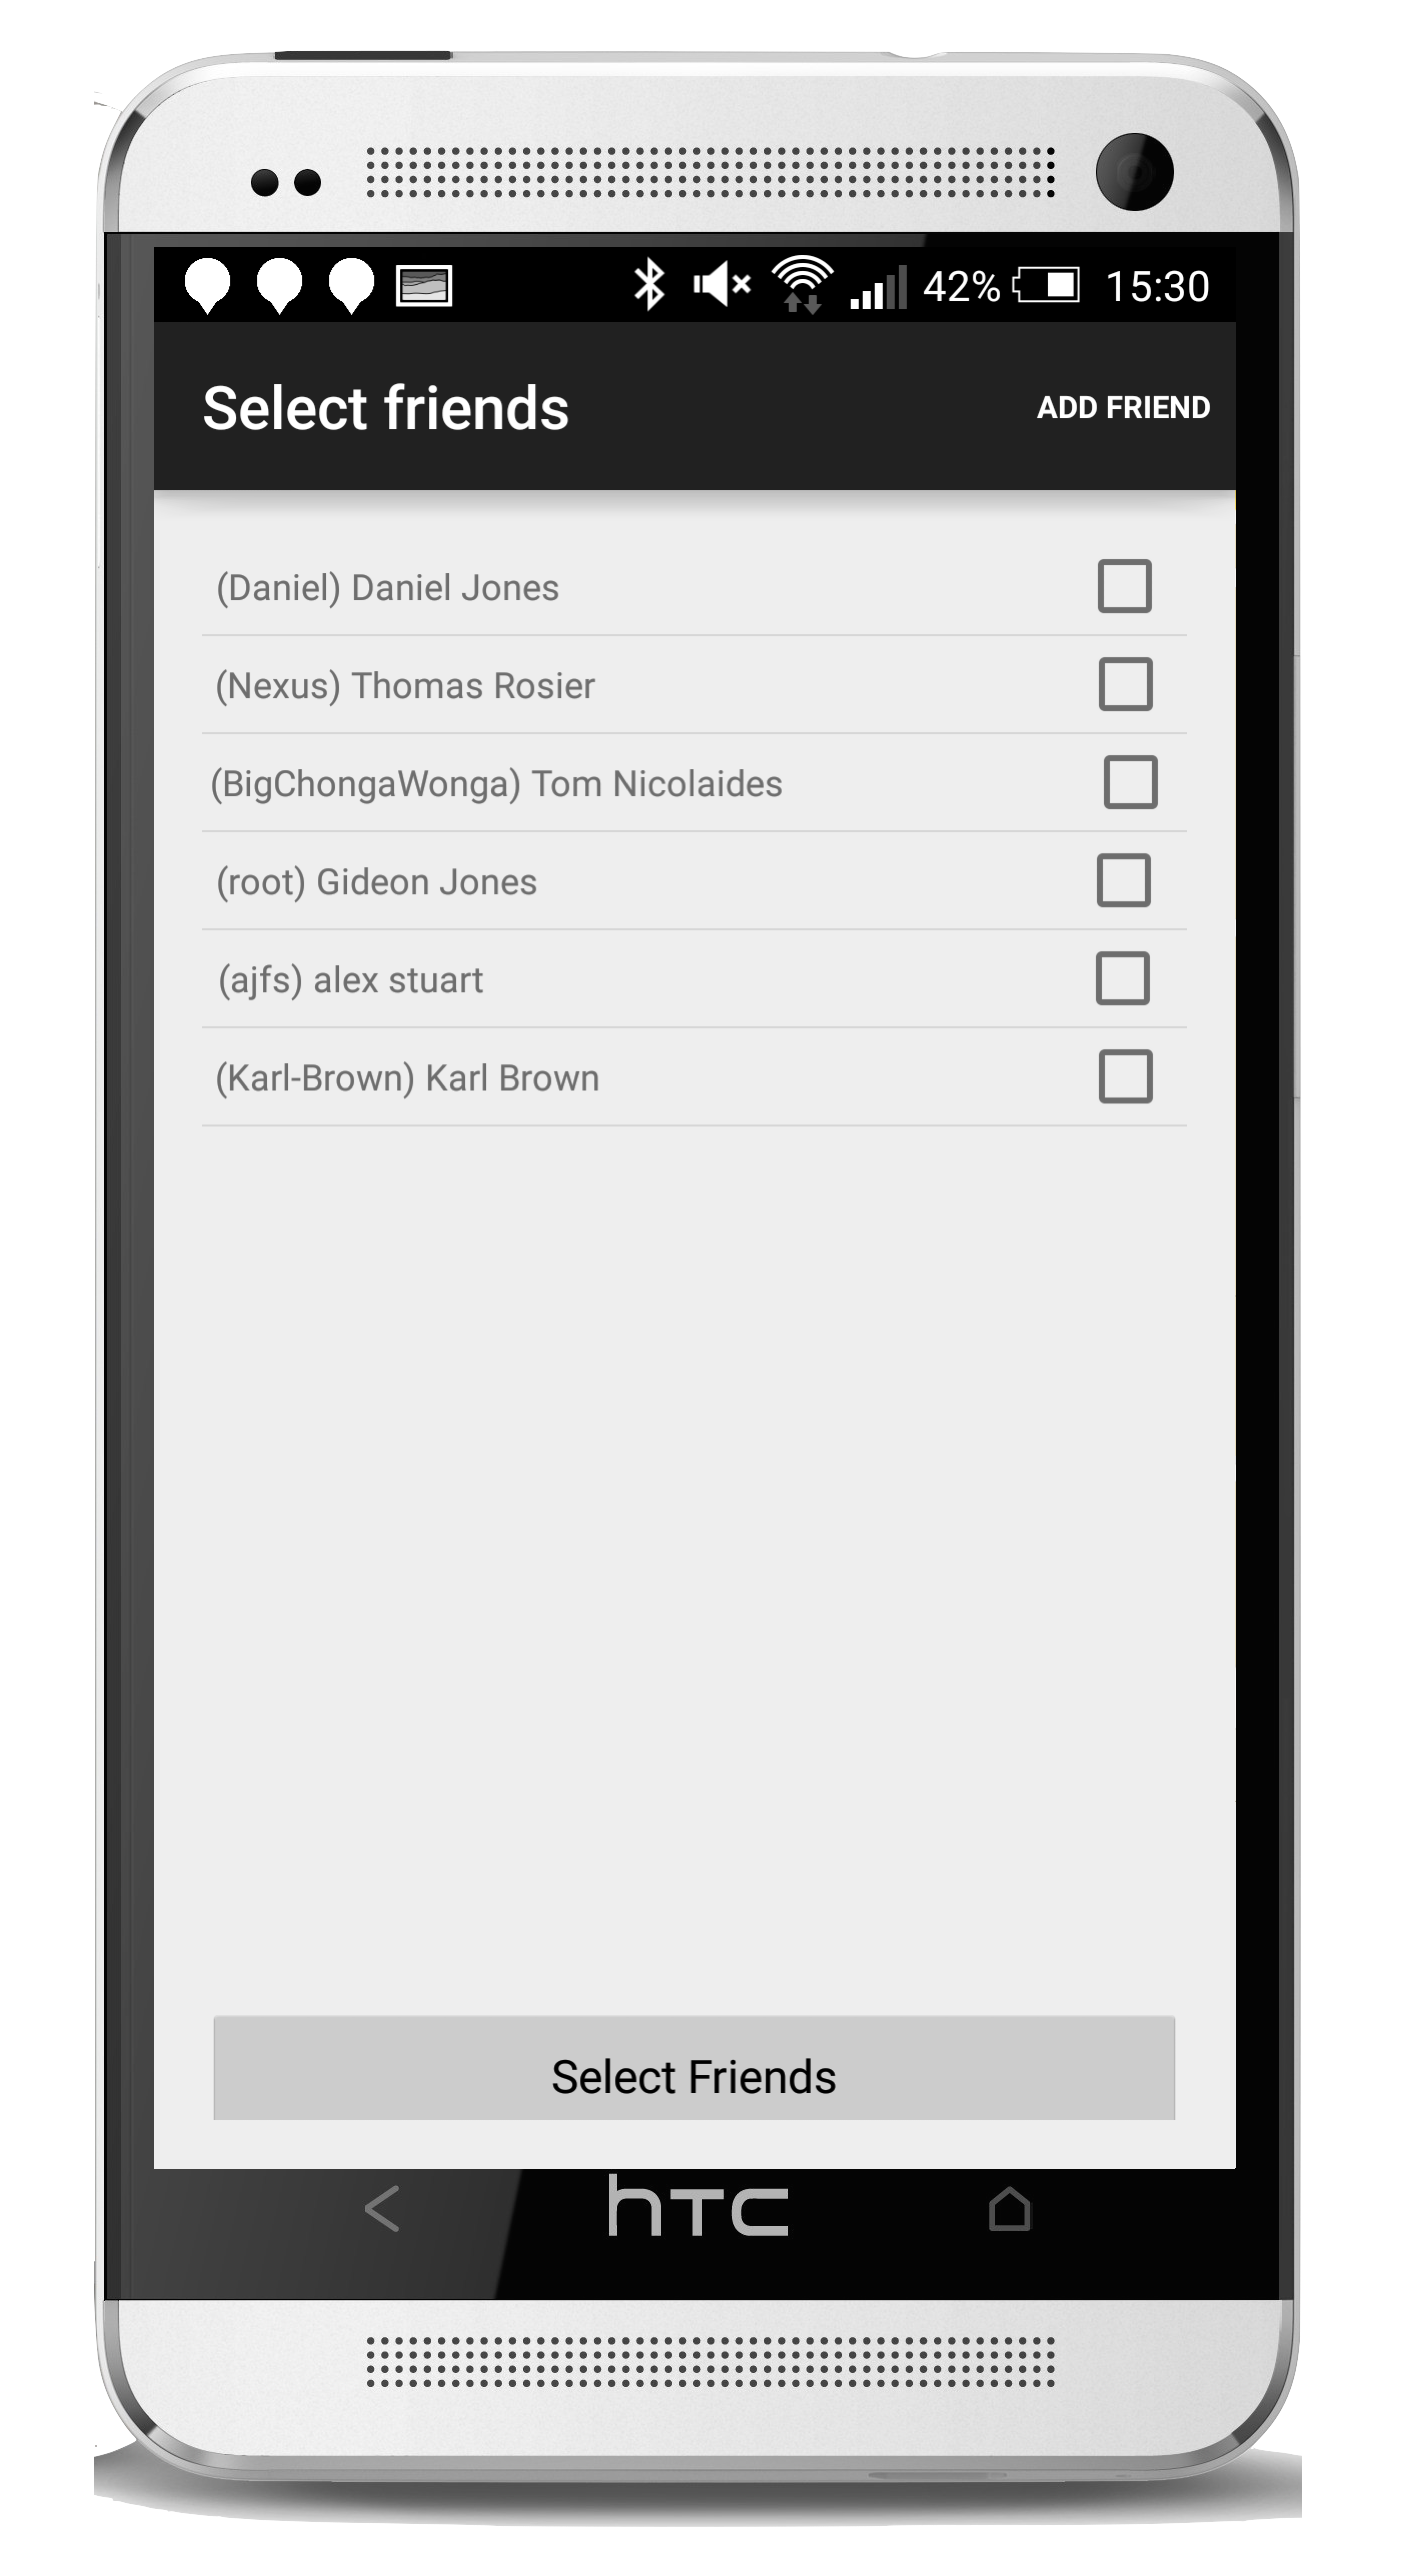
\includegraphics[width=\textwidth]{uiscaling/friends}
    \caption{Setting visibility to friends on different devices}
    \label{fig:ui_scaling_friends_image}
\end{figure} 
\noindent

\section{Functionality Testing}

\section{Stress Testing}

